\documentclass[10pt]{mypackage}

\usepackage{mlmodern}
%\usepackage{newpxtext,eulerpx,eucal}
%\renewcommand*{\mathbb}[1]{\varmathbb{#1}}

\usepackage{homework}
%\usepackage{notes}

%\usepackage[ backend=bibtex, style = alphabetic, sorting=ynt ]{biblatex}
%\addbibresource{  }

\usepackage{parskip}

\fancyhf{}
\fancyhead[R]{Avinash Iyer}
\fancyhead[L]{Algebraic Topology: Homework 19}
\fancyfoot[C]{\thepage}

\setcounter{secnumdepth}{0}

\begin{document}
\RaggedRight
\section{Revised Problems}%
\begin{problem}[Homework 17, Problem 1]
  Give two examples of a nontrivial covering space of the Klein bottle, one normal and one non-normal.
\end{problem}
\begin{solution}
  As discussed in the original submission, we observe that the torus can be viewed as a two-sheeted cover of the Klein bottle, and since the number of sheets is equal to the index of $p_{\ast}\left( \pi_1\left( \widetilde{X},\widetilde{x}_0 \right) \right)$ in $\pi_1\left( X,x_0 \right)$, we have that this is a normal cover.

  To find a non-normal cover, we consider the three-sheeted covering space given below. This covering space lifts the loop given by $a$ to three copies of itself, while it lifts $b$ to one copy of itself. In particular, its fundamental group corresponds to the subgroup of the Klein bottle group $\left\langle a,b|abab^{-1} \right\rangle$ given by $H = \left\langle a^3,b \right\rangle$. Yet, this subgroup is not normal since $b\in H$, but $aba^{-1} = a\left( aba \right)a^{-1} = a^2b\notin H$.
  \begin{center}
    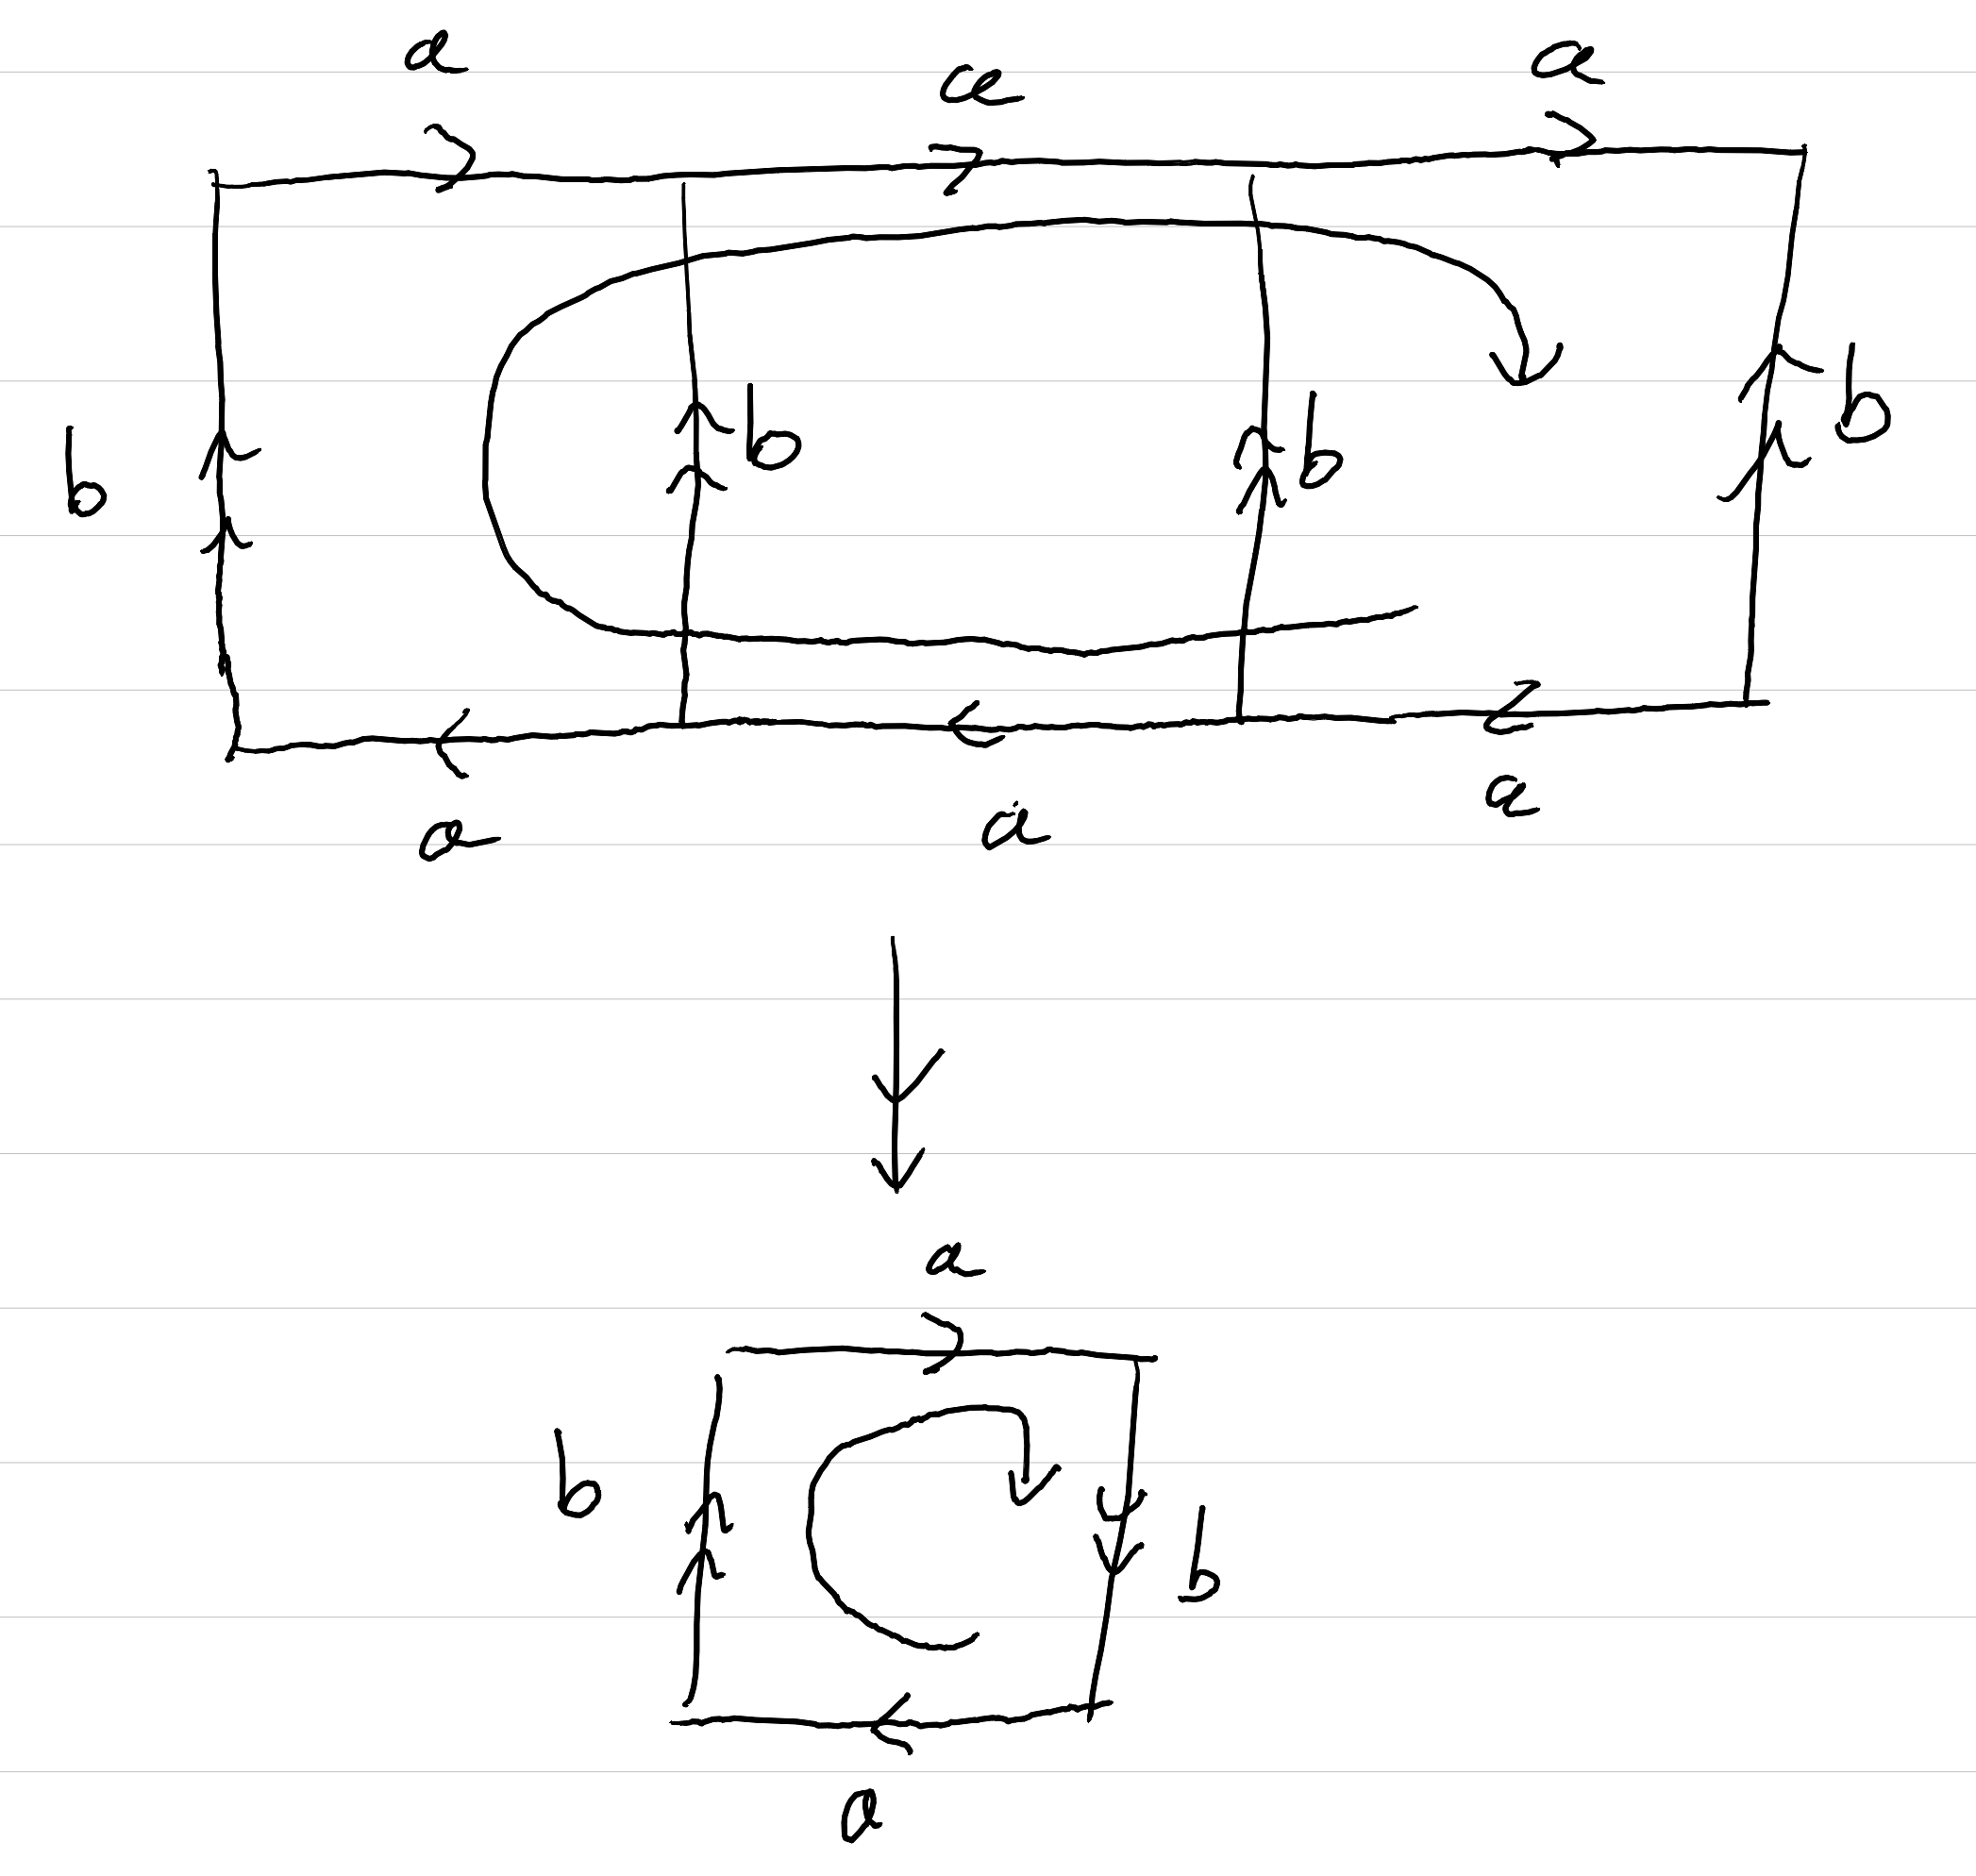
\includegraphics[width=10cm]{images/three_sheeted_klein_bottle.png}
  \end{center}
\end{solution}
\begin{problem}[Homework 17, Problem 2]
  Let $p\colon \widetilde{X}\rightarrow X$ be a covering space with $X$ path-connected, locally path-connected, and semilocally simply connected, but $\widetilde{X}$ is not necessarily path-connected. Prove that the path-components of $ \widetilde{X} $ are in bijection with the orbits of the action of $ \pi_1\left( X,x_0 \right) $ on the fiber $p^{-1}\left( x_0 \right)$.
\end{problem}
\begin{solution}
  We have that $\pi_1\left( X,x_0 \right)$ acts on the fiber $p^{-1}\left( x_0 \right)$ via lifting. That is, if $\gamma$ is a loop based at $x_0$ in $X$, then $\left[ \gamma \right]$ lifts to some path $ \widetilde{\gamma} $ taking $ \widetilde{x_0}\in p^{-1}\left( x_0 \right) $ to some point $ \widetilde{x_1} \in p^{-1}\left( x_0 \right)$, and the action takes $ \widetilde{x_0}\mapsto \widetilde{x_1} $.

  Suppose $Y$ is a path-component of $ \widetilde{X} $. We know that $\pi_1\left( X,x_0 \right)$ acts transitively on the restriction of the fiber $p^{-1}\left( x_0 \right)$ when restricted to $Y$, since a path-component of a covering space is a path-connected covering space. In particular, if $ \widetilde{x_0}\in p^{-1}\left( x_0 \right)\cap Y $ is any element, then the orbit of $ \widetilde{x_0} $ consists of all elements of $p^{-1}\left( x_0 \right)$ that are contained in $Y$. Since the orbit of any element of $p^{-1}\left( x_0 \right)$ is the path-component that element lies in, it follows that the orbits of the action are in one-to-one correspondence with the path-components of $\widetilde{X}$.
\end{solution}
\section{Current Problems}%
\begin{problem}[Problem 1]
  Compute the homology groups of
  \begin{align*}
    \underbrace{\mathbb{RP}^2\#\cdots\# \mathbb{RP}^2}_{g}
  \end{align*}
  for any $g\geq 1$.
\end{problem}
\begin{solution}
  We will label the surface as $X_g$. We know that $H_0\left( X_g \right)$ is equal to the direct sum of $\Z$ indexed by the path-components of $X$. Since $X_g$ has one path-component, we have $H_0\left(X_g\right) = \Z$.

  To compute $H_1$, we show that the connected sum of $g$ copies of $ \mathbb{RP}^2 $ can be equipped with the structure of a $2g$-sided polygon with sides identified cyclically, as in the following picture for $ \mathbb{RP}^2\# \mathbb{RP}^2 \# \mathbb{RP}^2 $.
  \begin{center}
    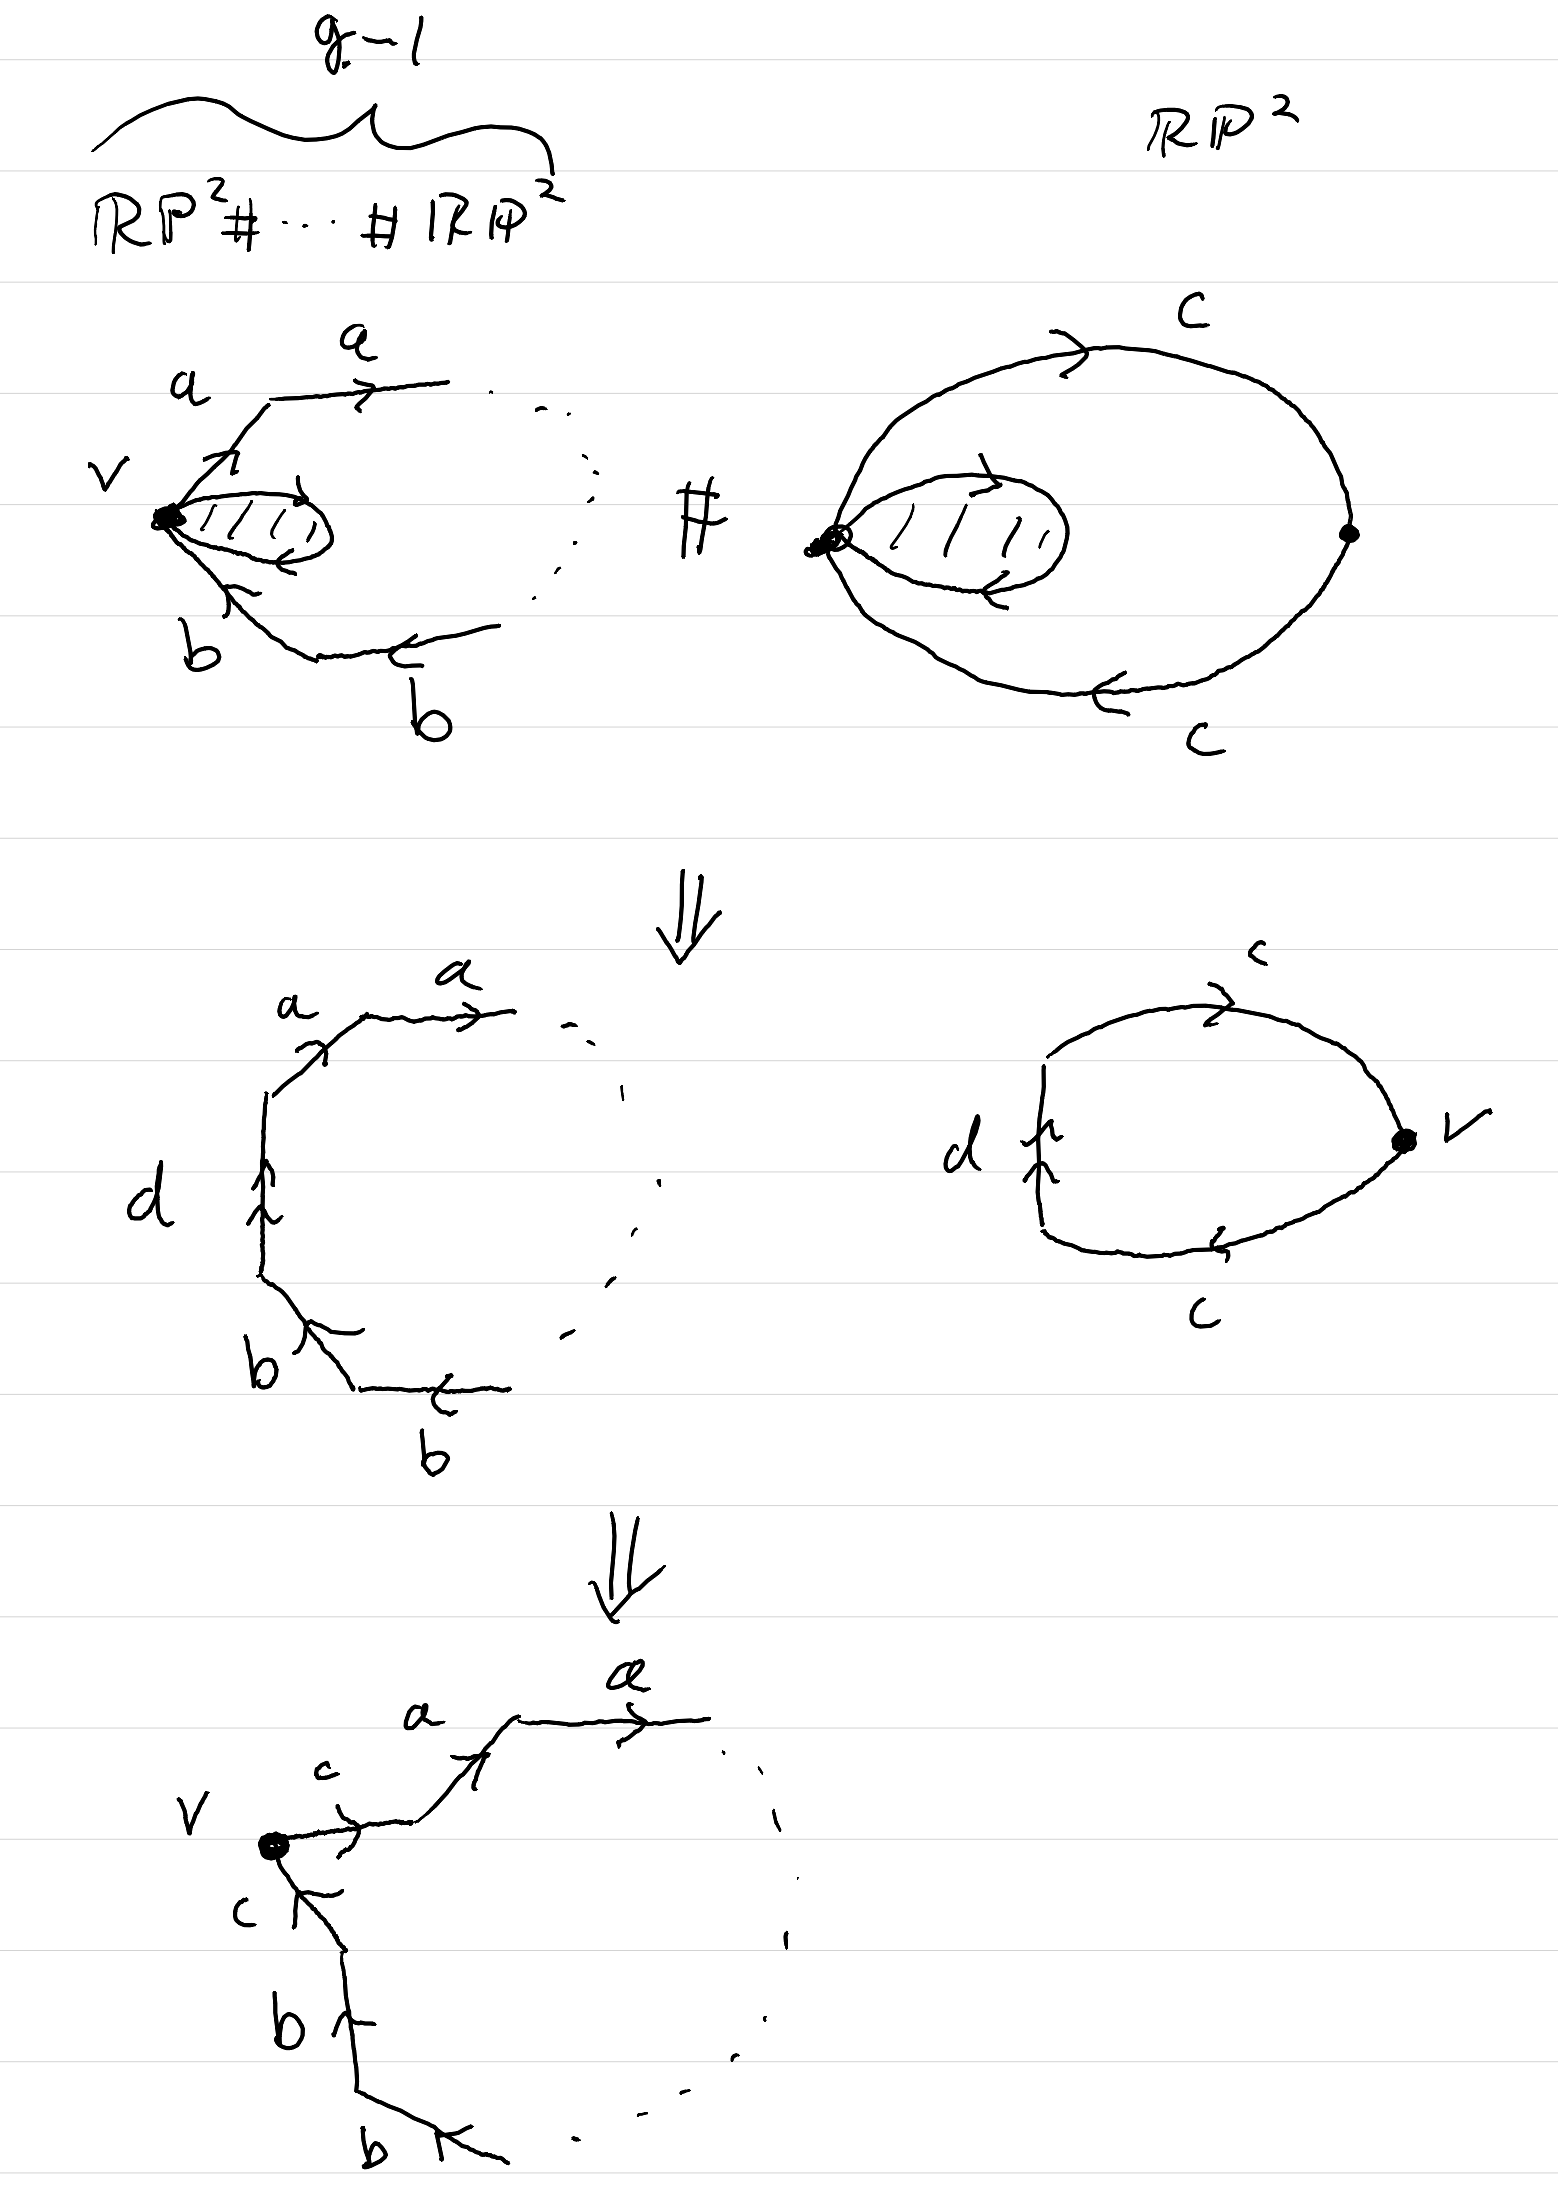
\includegraphics[width=10cm]{images/connected_sum_rp2.png}
  \end{center}
  If $v$ is the vertex in this connected sum, we may extract a copy of $D^2$ with its vertex at $v$, then observe that this attaches via the following connecting map to a copy of $ \mathbb{RP}^2 $. Since the base case is already satisfied by the definition of $ \mathbb{RP}^2 $ as its standard CW structure, we have our desired result.
  \begin{center}
    % https://tikzcd.yichuanshen.de/#N4Igdg9gJgpgziAXAbVABwnAlgFyxMJZABgBoBGAXVJADcBDAGwFcYkRiQBfU9TXfIRTkK1Ok1bsAwgH0ATAAoAGjIDmASm68QGbHgJE5omgxZtEIWeWVrNPPnsFEAzMfFnpM4jY1aHAgxQAFjdTSQtOex1+fSFkI2IxMPMQAB1UgCMsVQg0FjgZYCwAXnIuAD1gVS50gFt6HAALDIzgAC0uehksP2jHQORXRJMJFLqG5taOgAJaXt0AuJFh93C01PqmlvauaYAzeZinFCM5JNH2Lp6ohdiXUjORjwjD-qXSZ3PnkAObo4GjJ8nmtxlsplwFF1yABqdIAYygEBwcGhXV8XDEMCgqngRFAewAThBakgRCAcBAkEZVmNUmh6AS8Ex5L1CcSqTQKUhXDT2Ol6YysMzyKyiSTEDyuYgQryLPyGUzGF5RezEGRyZTEGTkny6QqhUrnCrxQAOTmagCcnPoWEY7HqaDgXKibPF5HVUvIZJwNrtFgdTspLrFSAA7ObSTRGFgwClEcwMow2DRGjB6FB2JBYyBrbbMwQ2MHVQBWCOIamp9P57NRmNxiAJpM58m+6uF7SupAANjLPMrGYsWeTIGj2Ys8cTw59ecHBe4lC4QA
\begin{tikzcd}
                          & \mathbb{Z} f \arrow[d, no head, Leftrightarrow] & \bigoplus_{i=1}^{g}\mathbb{Z}a_i \arrow[d, no head, Leftrightarrow] & \mathbb{Z} v \arrow[d, no head, Leftrightarrow] &   \\
0 \arrow[r, "\partial_3"] & C_2(X_g) \arrow[r, "\partial_2"]            & C_1(X_g) \arrow[r, "\partial_1"]                                & C_0(X_g) \arrow[r, "\partial_0"]            & 0 \\
                          &                                             & a_i \arrow[r, maps to]                                          & 0                                           &   \\
                          & f \arrow[r, maps to]                        & 2\mathbb{Z}(a_1+\cdots+a_g)                                      &                                             &  
\end{tikzcd}
  \end{center}
  In particular, this means that $C_1\left( X_g \right) = \bigoplus_{i=1}^{g}\Z a_{i}$. We observe that for each $a_i$, $\partial_1\left( a_i \right) = v-v = 0$, so that $\ker\left( \partial_1 \right) = C_1\left( X_g \right)$.

  Meanwhile, we observe that our face $f$ maps under the boundary map to $2\Z\left( a_1+\cdots+a_g \right)$. In particular, from some linear algebra, we find that
  \begin{align*}
    H_1\left( X_g \right) &= \left( \bigoplus_{i=1}^{g}\Z a_i \right)/\left( 2\Z\left( a_1+\cdots+a_g \right) \right)\\
                          &\cong \Z/2\Z \oplus \bigoplus_{i=1}^{g-1}\Z.
  \end{align*}
  As for $H_2$, since $\ker\left( \partial_2 \right) = 0$ and $\img\left( \partial_3 \right) = 0$, it follows that $H_2\left( X_g \right) = 0$.
\end{solution}
\begin{problem}[Problem 2]
  Combined with examples from class, we have computed the homology groups of all closed surfaces. What do you observe about the homology groups of orientable surfaces compared to non-orientable ones?
\end{problem}
\begin{solution}
  Orientable surfaces appear to have a nontrivial $2$-dimensional homology group, while non-orientable surfaces don't, while non-orientable surfaces have a copy of $\Z/2\Z$ in the $1$-dimensional homology group and have no nontrivial $2$-dimensional homology group.
\end{solution}
\end{document}
